\section{Voltage Regulator using 7805}
\subsection{Schematic design}
Students are proposed to capture the schematic design in Altium Designer and place the image in this part.

Some hot keys are normally used in the schematic is the space bar, X( horizontal mirror), Y (vertial mirror) and Ctrl + W (place a wire).

Your image goes here:

\begin{figure}[h]
    \centering
    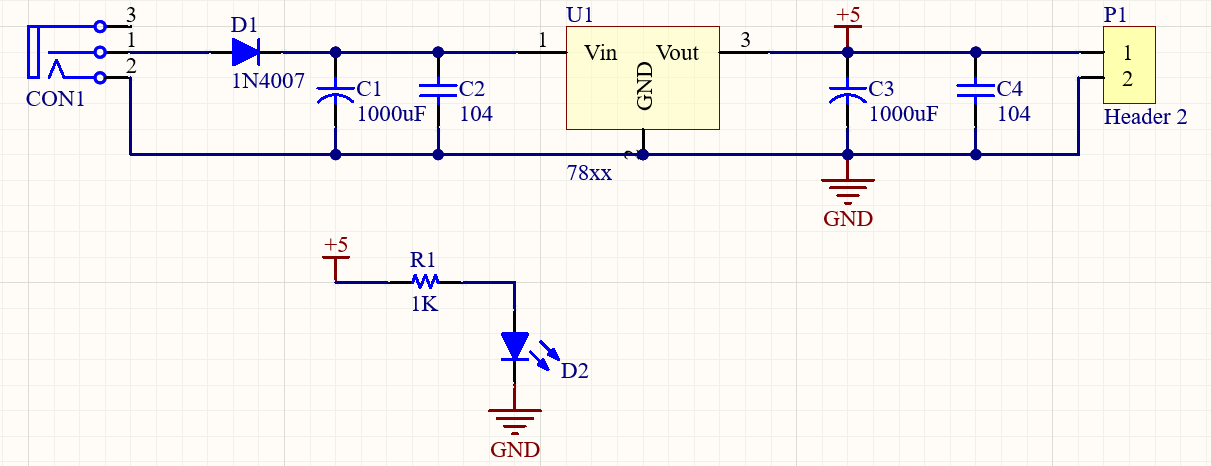
\includegraphics[width=0.9\textwidth]{graphics/ex1/f1.PNG}
\end{figure}

\subsection{PCB layout}
Similarly to the schematic, some snap shorts of for the TOP, BOTTOM layers are required in this report. Moreover, several 3D images of your schematic are also required.

Your image goes here:
\begin{figure}[h!bp]
    \centering
    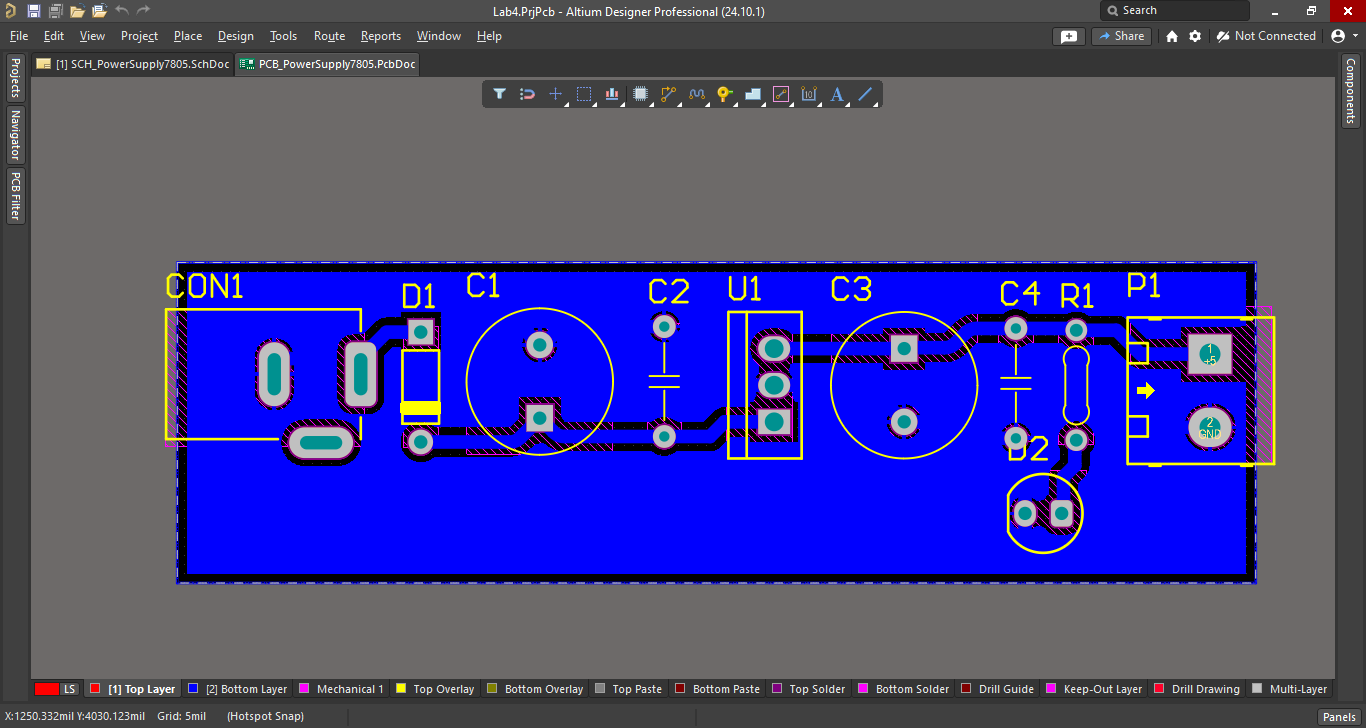
\includegraphics[width=0.6\textwidth]{graphics/ex1/f2.PNG}
    \caption{Top layer}
\end{figure}
\begin{figure}[t]
    \centering
    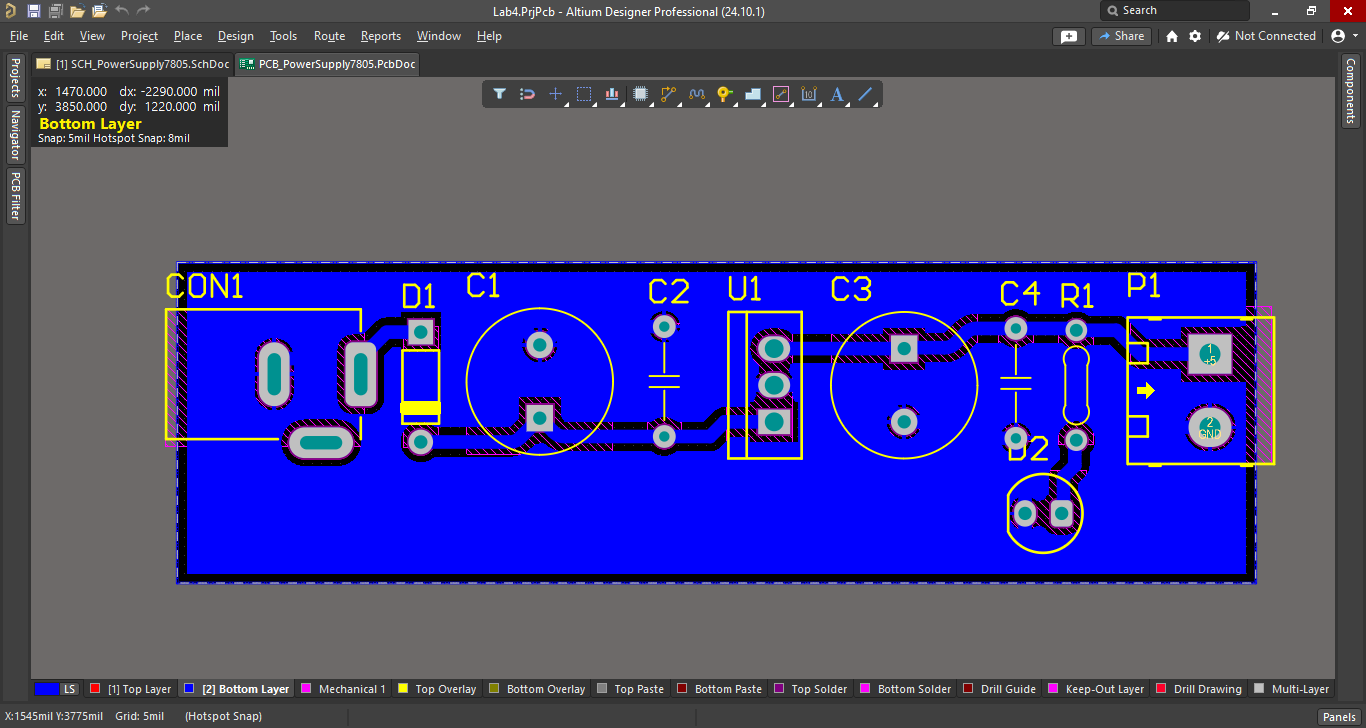
\includegraphics[width=0.6\textwidth]{graphics/ex1/f3.PNG}
    \caption{Bottom layer}
\end{figure}
\newpage
Several 3D images:
\begin{figure}[h]
    \centering
    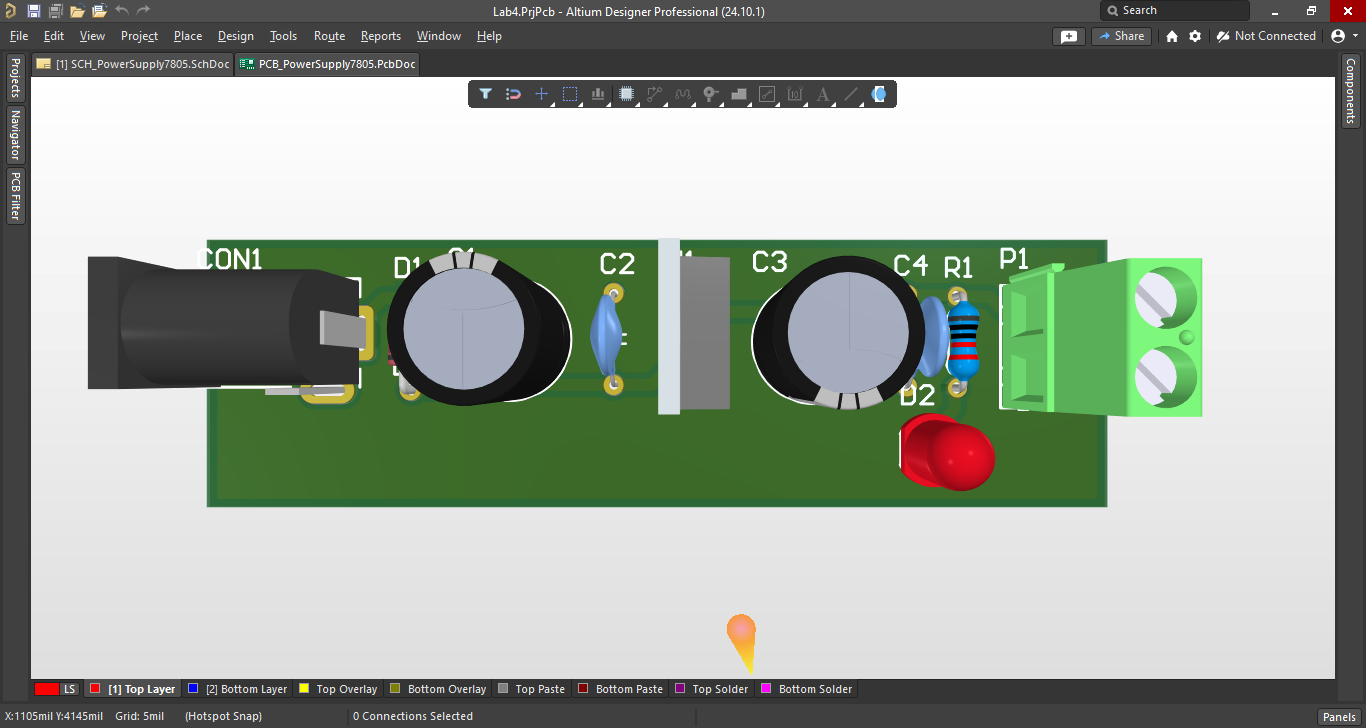
\includegraphics[width=0.6\textwidth]{graphics/ex1/f4.PNG}
    \caption{Top view}
\end{figure}
\begin{figure}[h!bp]
    \centering
    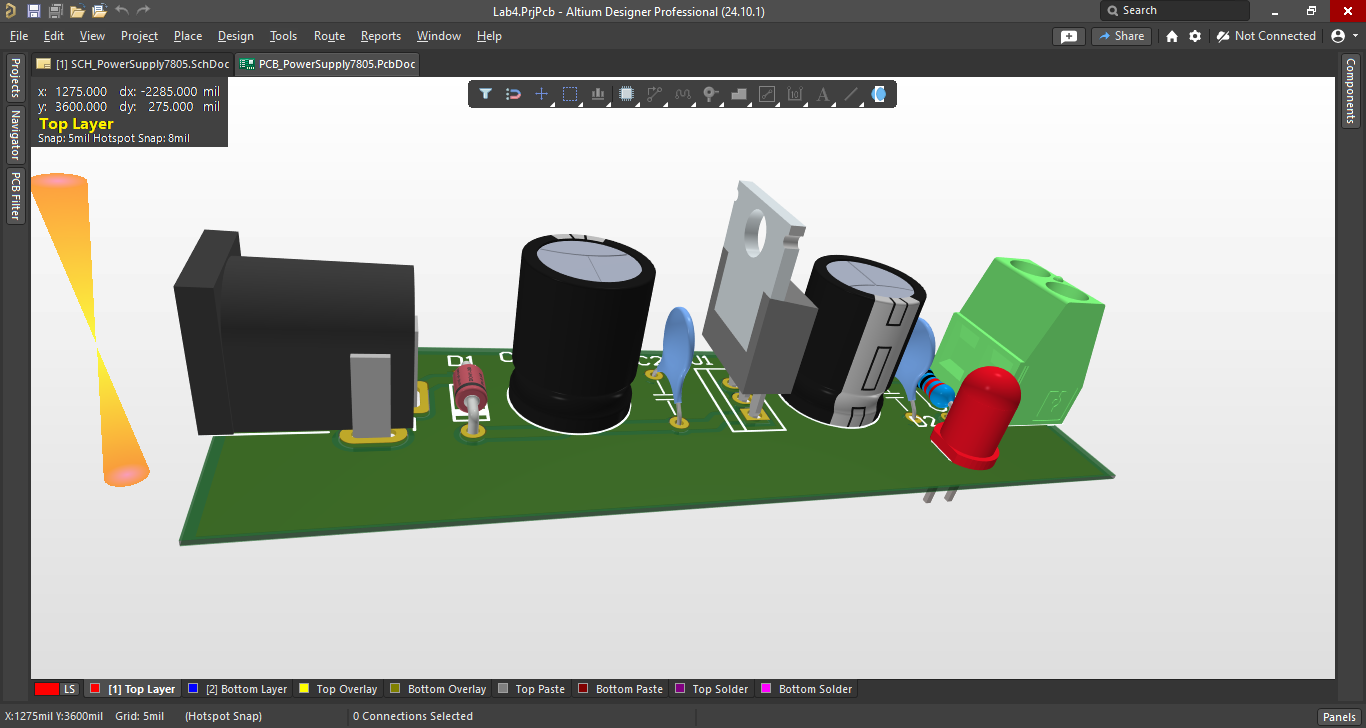
\includegraphics[width=0.6\textwidth]{graphics/ex1/f5.PNG}
    \caption{Beside view}
\end{figure}
% \FloatBarrier